%%%%%%%%%%%%%%%%%%%%%%%%%%%%%%%%%%%%%%%%%%%%%%%%%%%%%%%%%%%%%%%%%%%%%%
% LaTeX Template: Beamer arrows
%
% Source: http://www.texample.net/
% Feel free to distribute this template, but please keep the
% referal to TeXample.net.
% Date: Nov 2006
% 
%%%%%%%%%%%%%%%%%%%%%%%%%%%%%%%%%%%%%%%%%%%%%%%%%%%%%%%%%%%%%%%%%%%%%%
% How to use writeLaTeX: 
%
% You edit the source code here on the left, and the preview on the
% right shows you the result within a few seconds.
%
% Bookmark this page and share the URL with your co-authors. They can
% edit at the same time!
%
% You can upload figures, bibliographies, custom classes and
% styles using the files menu.
%
% If you're new to LaTeX, the wikibook is a great place to start:
% http://en.wikibooks.org/wiki/LaTeX
%
%%%%%%%%%%%%%%%%%%%%%%%%%%%%%%%%%%%%%%%%%%%%%%%%%%%%%%%%%%%%%%%%%%%%%%

\documentclass[handout]{beamer} %
\usetheme{CambridgeUS}
\usepackage[latin1]{inputenc}
\usefonttheme{professionalfonts}
\usepackage{times}
\usepackage{tikz}
\usepackage{amsmath}
\usepackage{verbatim}
\usetikzlibrary{arrows,shapes}
\beamertemplatenavigationsymbolsempty

\AtBeginSection[]{
\frame{\frametitle{}
\tableofcontents[current]}
}

\author[]{Shao Group Meeting}
\institute[]{University of Oklahoma }
\title[Machine Learning]{Machine Learning in Computational Chemistry}
\date[November 14, 2017]{November 14, 2017}

\begin{document}

\begin{comment}
:Title: Beamer arrows
:Tags: Remember picture, Beamer, Physics & chemistry, Overlays
:Use page: 3

With PGF/TikZ version 1.09 and later, it is possible to draw paths between nodes across
different pictures. This is a useful feature for presentations with the
Beamer package. In this example I've combined the new PGF/TikZ's overlay feature
with Beamer overlays. Download the PDF version to see the result.
**Note.** This only works with PDFTeX, and you have to run PDFTeX twice.
| Author: Kjell Magne Fauske

\end{comment}


% For every picture that defines or uses external nodes, you'll have to
% apply the 'remember picture' style. To avoid some typing, we'll apply
% the style to all pictures.
\tikzstyle{every picture}+=[remember picture]

% By default all math in TikZ nodes are set in inline mode. Change this to
% displaystyle so that we don't get small fractions.
\everymath{\displaystyle}

\frame{\titlepage}

\section{ML Prediction of Total Energy and Components} 

\subsection{Total HK DFT Energies, Mueller (2017)}

\begin{frame}
\begin{center}
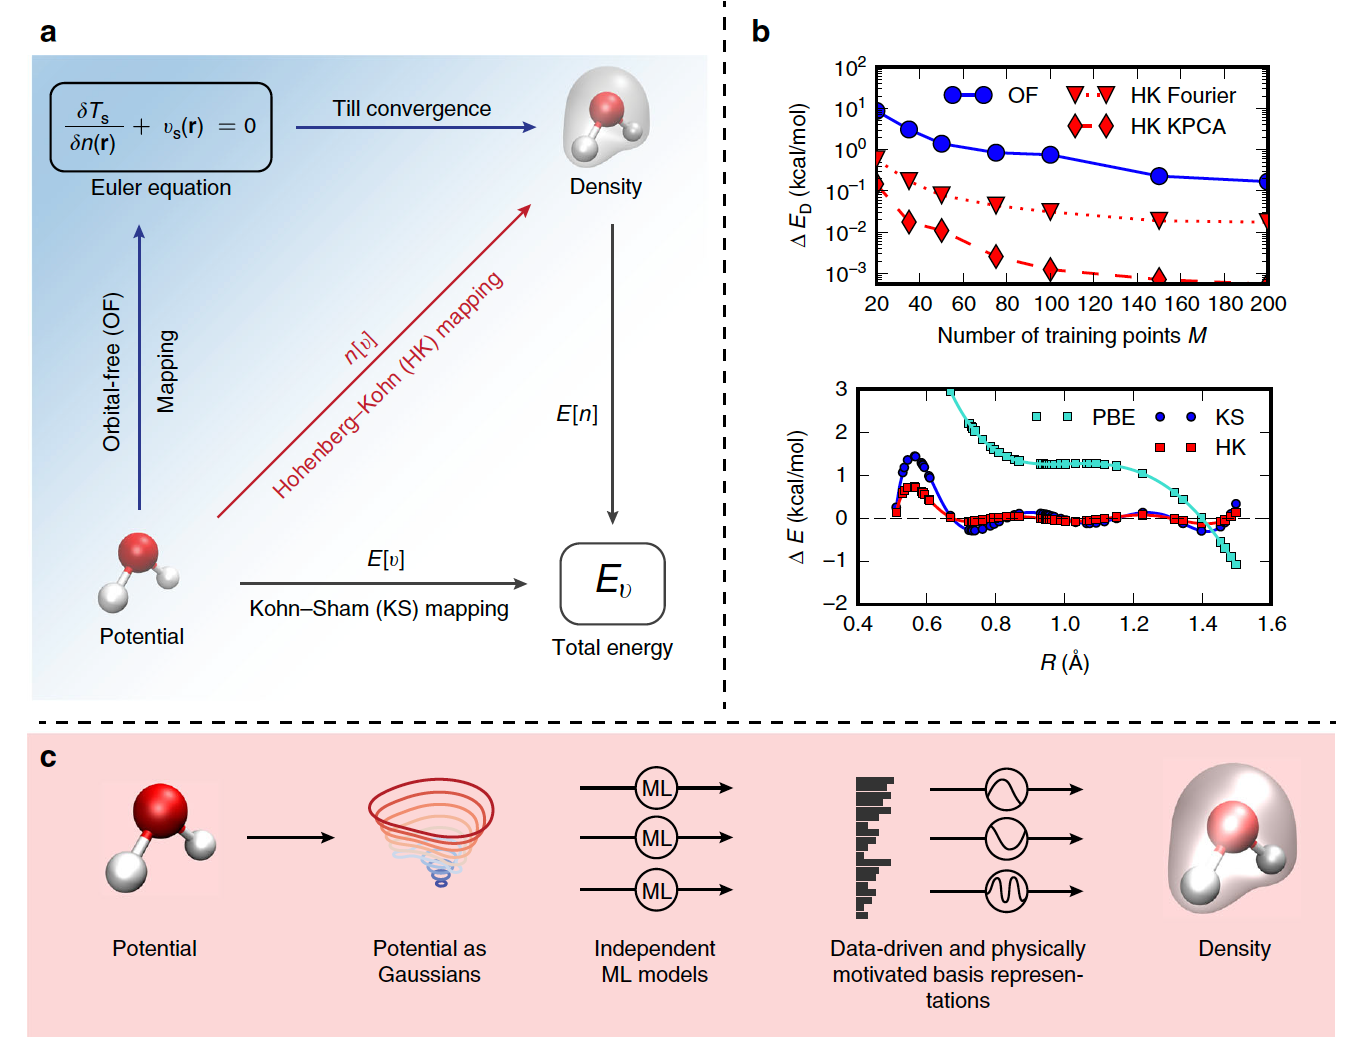
\includegraphics[height=2.6in]{figures_ml/Mueller_summary.png}
\end{center}
\vspace{1mm}
\begin{center}
\footnotesize{Brockherde, Vogt, Li, Tuckerman, Burke and Mueller, Nat. Commun. 8, 872 (2017).}
\end{center} 
\end{frame}

\begin{frame}
\begin{center}
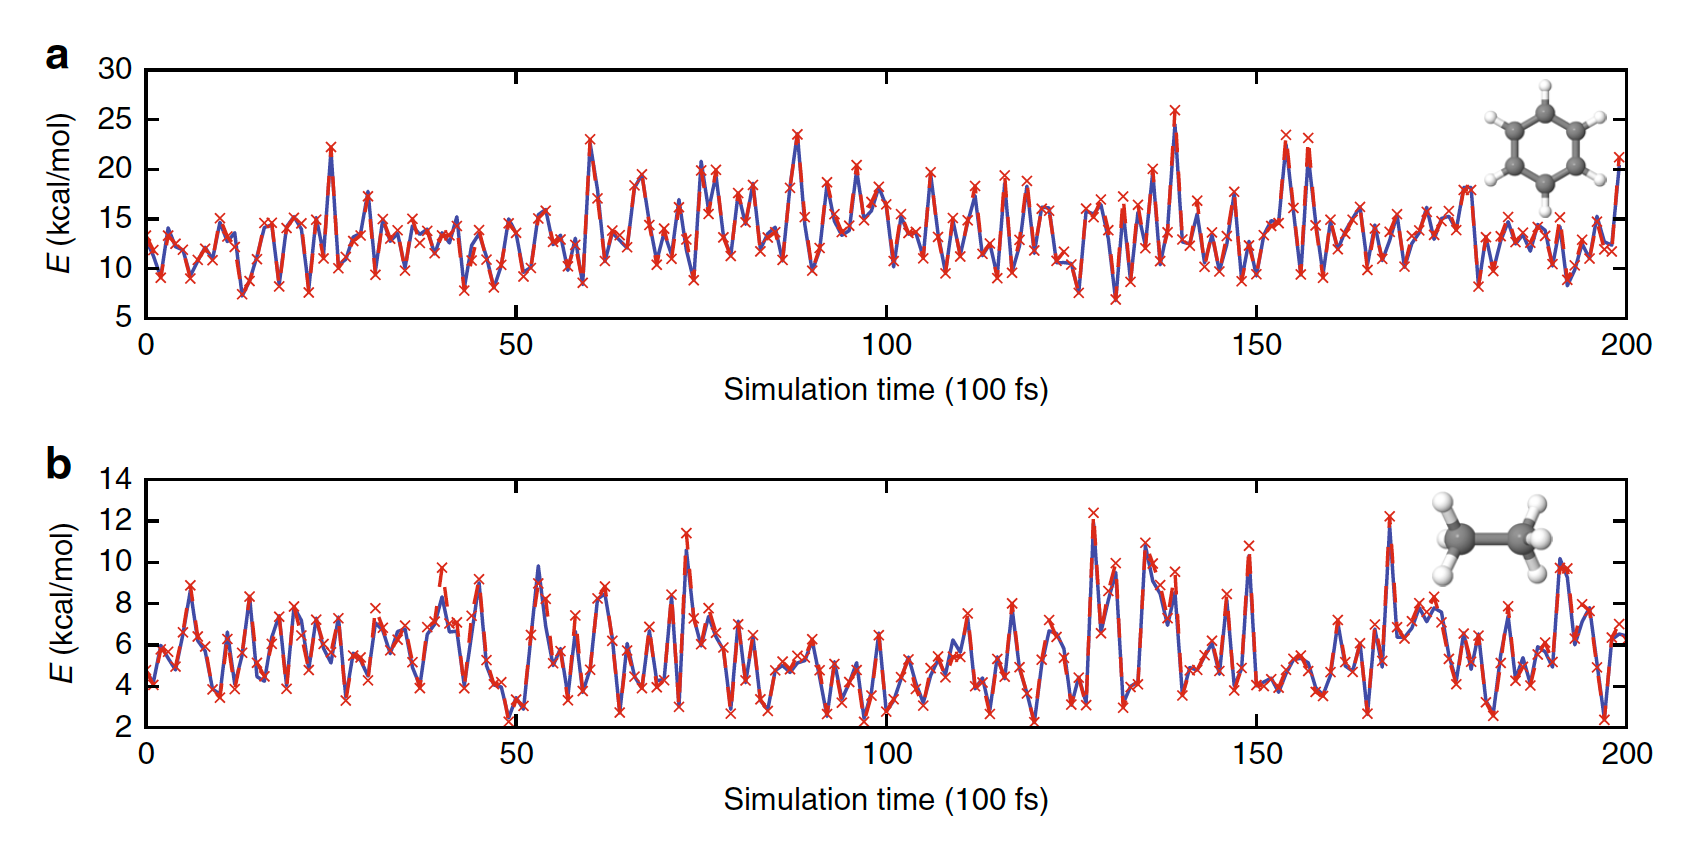
\includegraphics[height=2.4in]{figures_ml/Mueller_benzene_ethane.png} \\
\textcolor{blue}{Blue: PBE;}  \textcolor{red}{Red: ML-HK}
\end{center}
\vspace{5mm}
\begin{center}
\footnotesize{Brockherde, Vogt, Li, Tuckerman, Burke and Mueller, Nat. Commun. 8, 872 (2017).} 

\end{center} 
\end{frame}

\begin{frame}
\begin{center}
\includegraphics[height=2.4in]{figures_ml/Mueller_malonaldehyde.png} \\
\textcolor{blue}{Blue: PBE;}  \textcolor{red}{Red: ML-HK}
\end{center}
\vspace{5mm}
\begin{center}
\footnotesize{Brockherde, Vogt, Li, Tuckerman, Burke and Mueller, Nat. Commun. 8, 872 (2017).}
\end{center} 
\end{frame}

\subsection{Total DFT Energy, Roitberg (2017)} 

\begin{frame}
\begin{center}
\includegraphics[height=2.4in]{figures_ml/Roitberg_nn.png}
\end{center}
\vspace{5mm}
\begin{center}
\footnotesize{Smith, Isayev, and Roitberg, Chem. Sci., 8, 3192 (2017).}
\end{center} 
\end{frame}

\begin{frame}
\begin{itemize}
\item \scriptsize{Working equations}
\begin{eqnarray*}
E_{total} & = & \sum_{i} E_i   \\
G_i^R & = & \sum_{j \neq i} ^{N} e^{-\eta ( R_{ij} - R_s ) ^2 } f_c ( R_{ij} )  \\
G_m^{\textrm{mod}} & = & 2 ^ { 1-\xi} \sum_{j, k \neq i}   \left[ 1 + cos (\theta_{ijk} - \theta_s) \right]^ \xi 
e^ { - \eta \left( \frac{R_{ij} + R_{jk}} {2} - R_s \right)^2 } f_c  ( R_{ij} )  f_c  ( R_{ik} )    \\
f_c (R) &  = &  \left\{ \begin{array}{l}  0.5 cos \left( \pi R / Rc \right) + 0.5,~~~~ R \leq R_c \\ 0  \end{array} \right.   \\
\end{eqnarray*}
\item Training set: 57951 molecules.  Up to 8 ``heavy atoms" (C, N, O) from GDB-11 database 
\item $>$ 3N-6 structures for each molecule.   $\sim$ 17.2 million structures in total.   
\item Target data: $\omega$B97X/6-31G* energies.  
\item Number of nodes: 768: 128 : 128 : 64 : 1
\end{itemize}
\vspace{5mm}
\begin{center}
\footnotesize{Smith, Isayev, and Roitberg, Chem. Sci., 8, 3192 (2017).}
\end{center} 
\end{frame}


\begin{frame}
\begin{center}
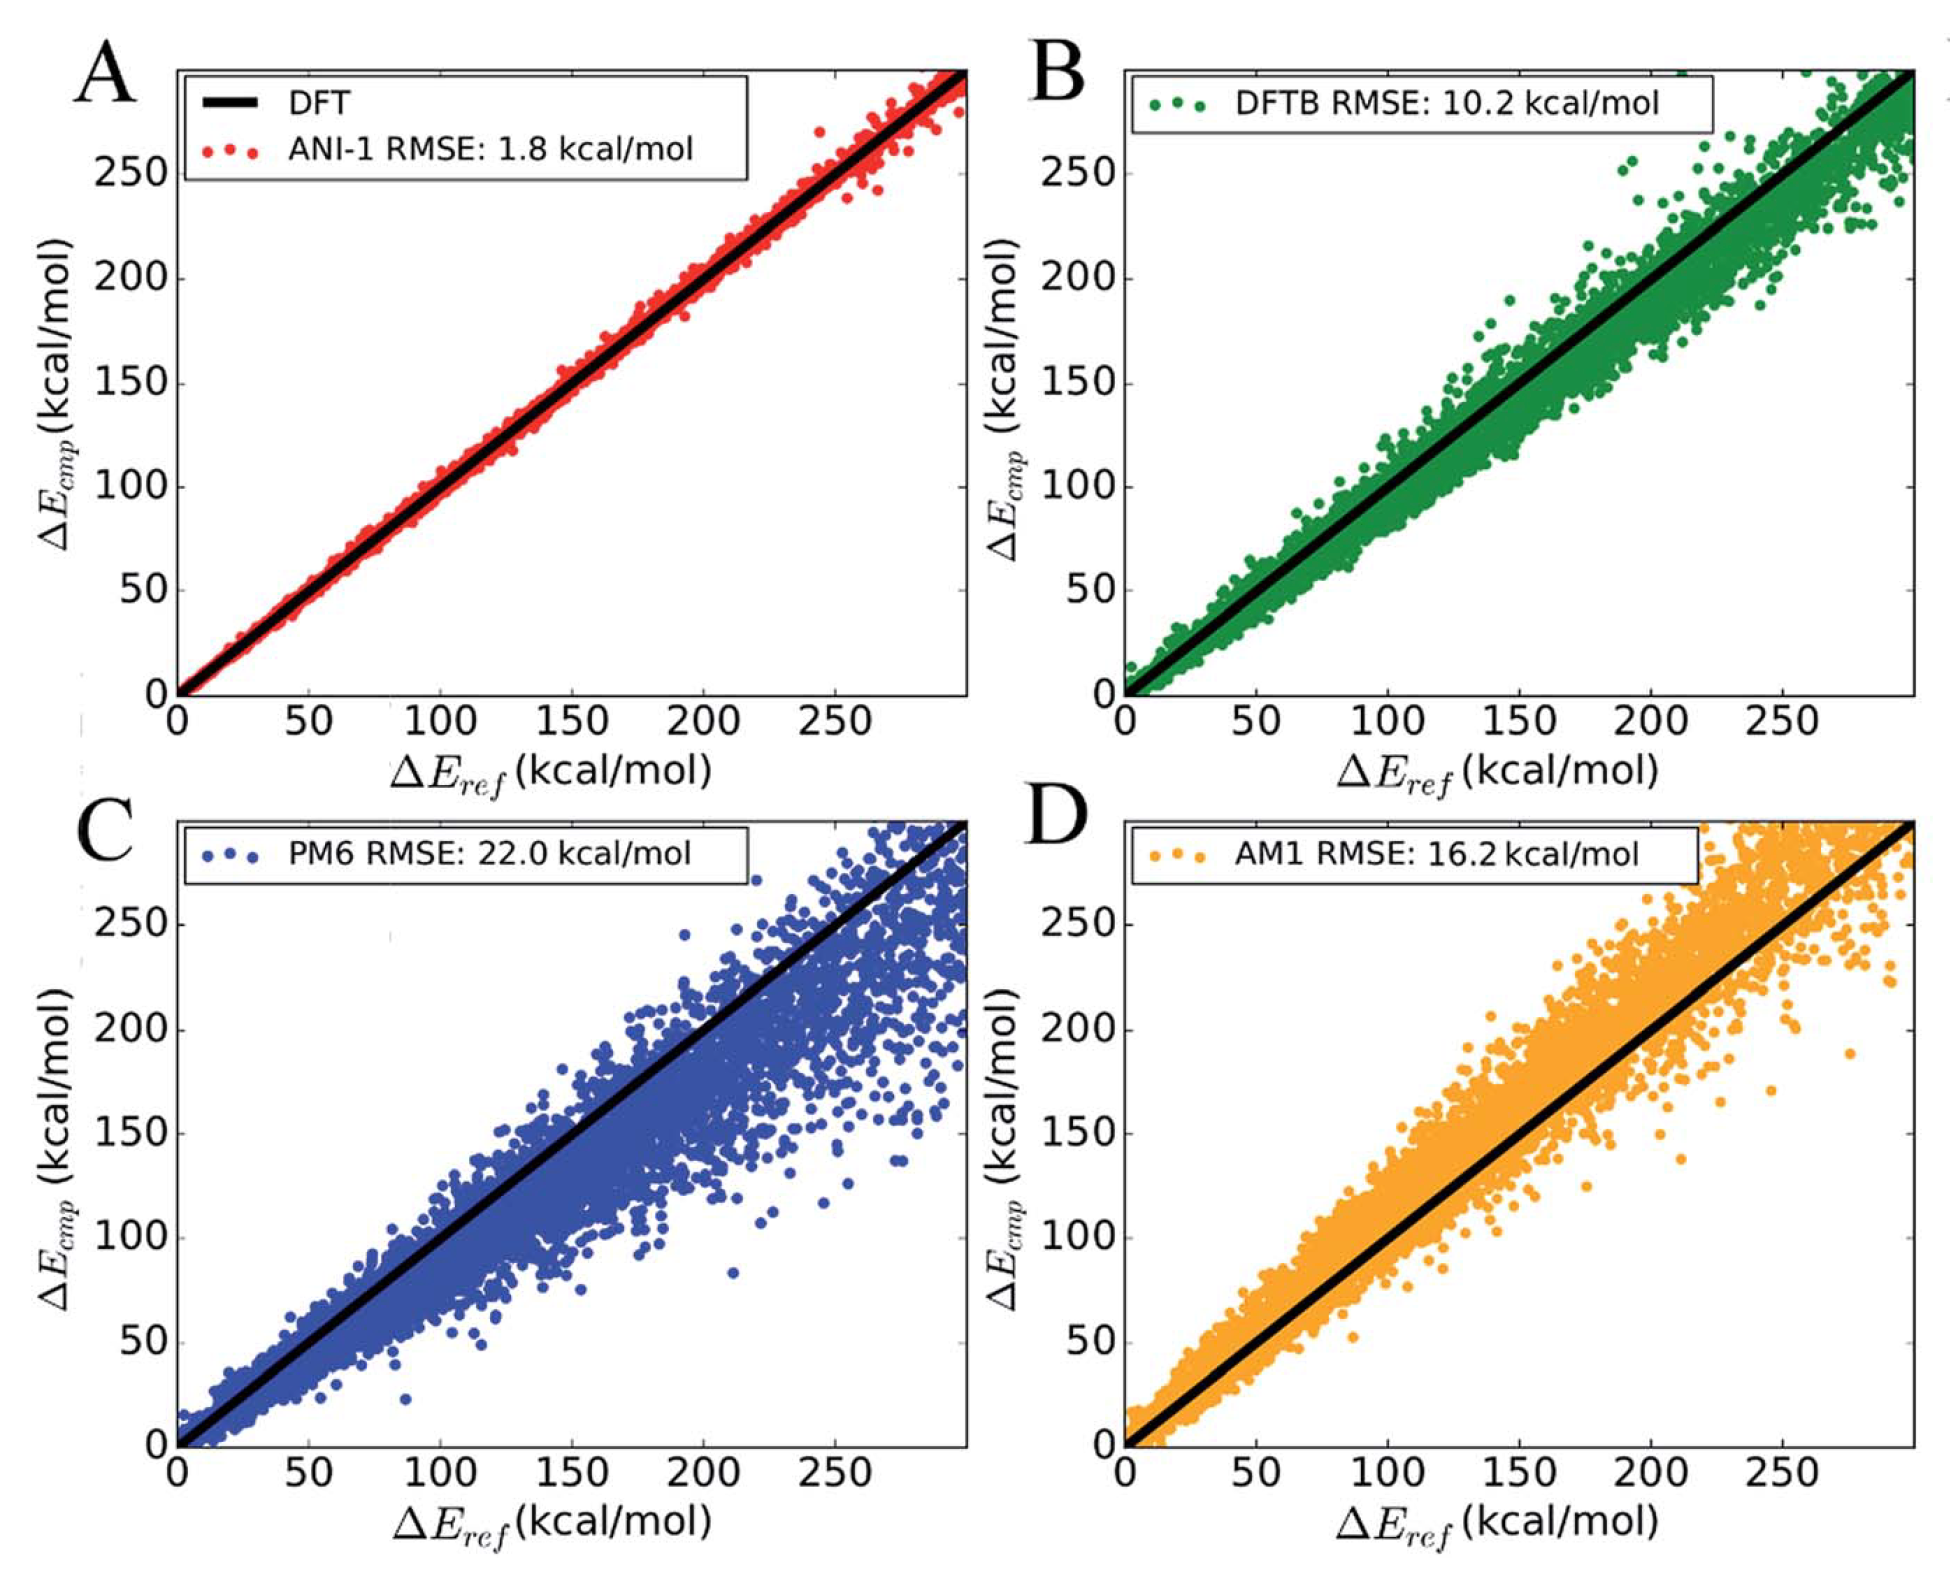
\includegraphics[height=2.4in]{figures_ml/Roitberg_scatter.png}
\end{center}
\vspace{5mm}
\begin{center}
\footnotesize{Smith, Isayev, and Roitberg, Chem. Sci., 8, 3192 (2017).}
\end{center} 
\end{frame}

\subsection{1-Body, 2-Body, and 3-Body Energies, Parkhill (2016)}

\begin{frame}
\begin{itemize}
\item \footnotesize{Many-body expansion}
\begin{eqnarray*}
E_{total} & = & \sum_{i} E_i + \sum_{i < j} \Delta E_{ij} + \sum_{ i < j < k } \Delta E_{ijk} \\
\Delta E_{ij} & = & E_{ij} - E_i - E_j \\
\Delta E_{ijk} & =  & E_{i,j,k} - \Delta E_{ij} - \Delta E_{ik} - \Delta_{jk} - E_i - E_j - E_k 
\end{eqnarray*}
\item Machine learning 
\begin{itemize}
\item \footnotesize{1-body: one hidden layer NN, 50 000 neurons, 844 800 samples}
\item 2-body: two hidden layers, 10 000 + 5000 neurons, 74240 samples
\item 3-body: three hidden layers, 1000 + 2000 + 2000 Neurons, 36 864 samples  
\item samples from MD trajectory of 108 methanol molecules
\item \textcolor{red}{Permutational invariance} is considered. 
\end{itemize}

\end{itemize}

\vspace{10mm}
\begin{center}
\footnotesize{Yao, Herr, Parkhill, JCP, 146, 014106 (2016).}
\end{center} 
\end{frame}


\begin{frame}
\begin{center}
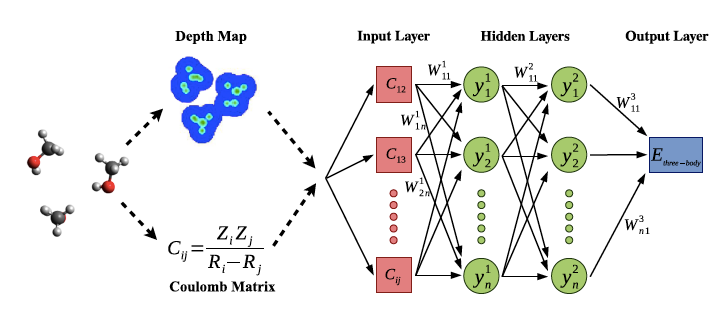
\includegraphics[height=1.8in]{figures_ml/parkhill_nn.png}
\end{center}
\vspace{10mm}
\begin{center}
\footnotesize{Yao, Herr, Parkhill, JCP, 146, 014106 (2016).}
\end{center} 
\end{frame}

\begin{frame}
\begin{center}
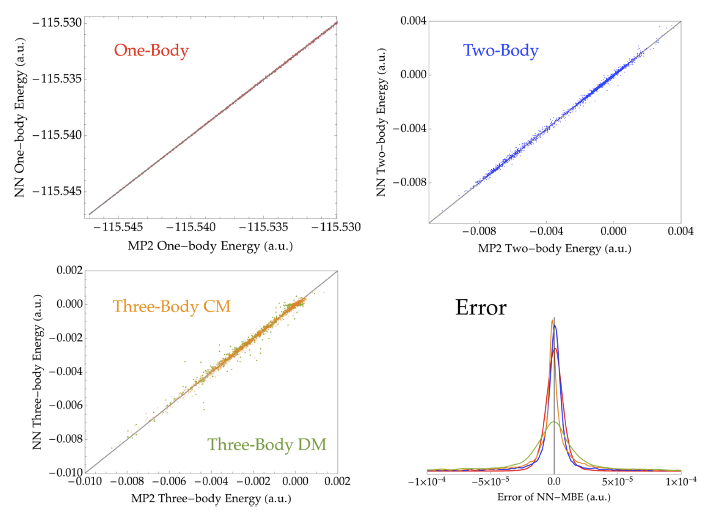
\includegraphics[height=2.8in]{figures_ml/parkhill_scatter.png}
\end{center}

\vspace{-1mm}
\begin{center}
\footnotesize{Yao, Herr, Parkhill, JCP, 146, 014106 (2016).}
\end{center} 
\end{frame}


\begin{frame}
\vspace{-3mm}
\begin{table}
\caption{Errors in kcal/mol} 
\begin{tabular}{lcccc}
\hline \hline 
Error  & 1-body & 2-body & 3-body (CM) & 3-body (DM) \\
\hline 
MSE & 0.0002 & 0.0006 & -0.0007 & -0.0025 \\
MAE & 0.0038 & 0.0098 & 0.0126 & 0.0244 \\
\hline \hline 
\end{tabular}
\end{table}

\begin{center}
%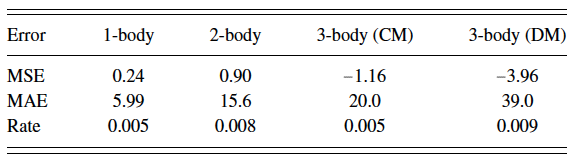
\includegraphics[height=0.6in]{figures_ml/parkhill_rms.png} \\
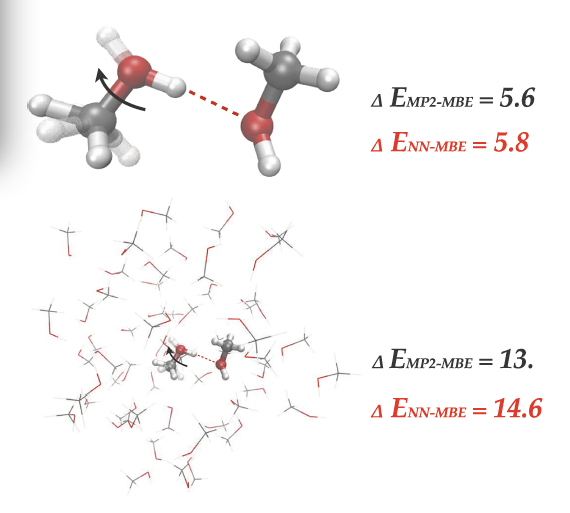
\includegraphics[height=2.2in]{figures_ml/parkhill_methanol_dimer.png} 
\end{center}
\vspace{5mm}
\begin{center}
\footnotesize{Yao, Herr, Parkhill, JCP, 146, 014106 (2016).}
\end{center} 
\end{frame}

\section{ML Prediction of Energy Differences} 

\subsection{E(aiQM) - E(SQM), Weitao Yang (2016, 2017)}

\begin{frame}
\begin{itemize}
\item \scriptsize{Working equations are}
\begin{eqnarray}
E_i & = & \sum_{j=1}^L w_{ij} ~\mathrm{tanh} \left(  w_{ij1} G_i^1 + w_{ij2} G_i^2  + w_{ij3} Q_i  + b_{ij} \right) + b_i  \\
G_i^1 & = & \sum_{j \neq i} ^{N} e^{-\eta ( R_{ij} - R_s ) ^2 } f_c ( R_{ij} ) \\
G_i^2 & = & 2 ^ { 1-\xi} \sum_{j, k \neq i}  ^ N ( 1 \pm cos \theta_{ijk} ) ^ \xi e ^ { - \eta ( R_{ij}^2 + R_{jk}^2 + R_{ik}^2 }  f_c  ( R_{ij} )  f_c  ( R_{jk} )  f_c  ( R_{ik} )   \\
f_c (R) &  = &  \left\{ \begin{array}{l}  0.5 cos \left( \pi R / Rc \right) + 0.5,~~~~ R \leq R_c \\ 0  \end{array} \right.   \\
\Delta E_{RC} & = & \sum_{j=1}^L w_{j}'~\mathrm{tanh} \left(  w_{j1}' z + w_{j2}' A(z)  + w_{j3}'  \frac{\partial A(z)}{\partial z}   + b_{j}' \right) + b' \\  
\Delta E & = & \sum_i^N \Delta E_i + \Delta E_{RC} 
\end{eqnarray}
\item Parameters: $R_c$ = 6\AA; $R_s$ = 0; $\eta$ = 0.09 - 1.80; $\xi$ = 0.09-1.80. 
\item Size of training set: 20 (S$_N$2); 20 (glycine in water); 30 (Claisen rearrangement)
\end{itemize}

\end{frame}

\begin{frame}
\begin{itemize}
\item Work flow
\begin{center}
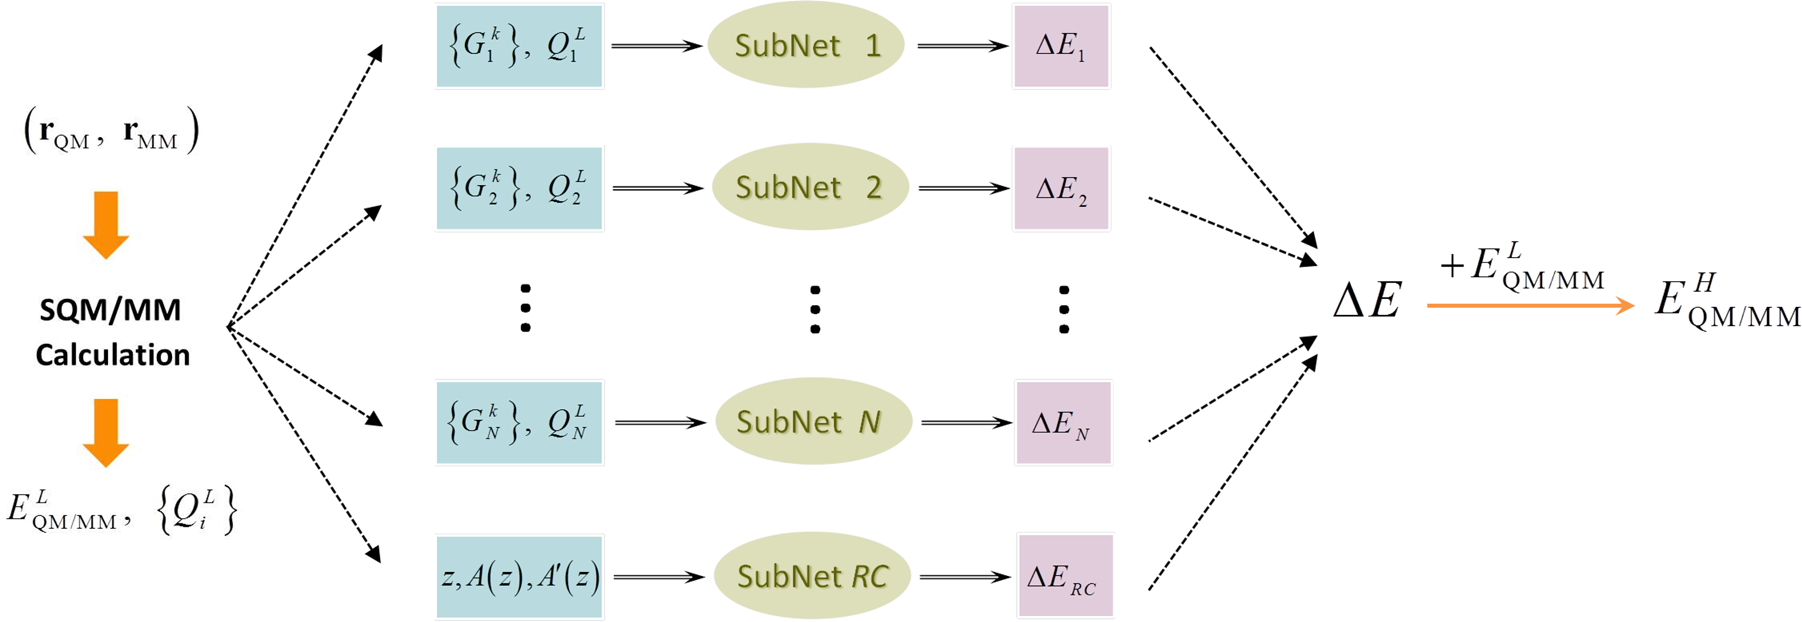
\includegraphics[height=1.5in]{figures_ml/weitao_1.png}
\end{center}
%\item Model details
\item \footnotesize{The final free energy profile is computed with}
\begin{eqnarray}
\Delta A^H_{z_1 \rightarrow z_2} & = &  \Delta A^L_{z_1 \rightarrow z_2}  + \Delta A^{L \rightarrow H} (z_2) -  \Delta A^{L \rightarrow H} (z_1) \\
\Delta A^{L \rightarrow H} (z) & = & - \beta^{-1} ~\mathrm{ln} \left< e^{ - \beta (E^H - E^L) } \right>_z 
\end{eqnarray}
\item Shen, Wu, Yang, JCTC, 12, 4934 (2016). 
\end{itemize}
\end{frame}

\begin{frame}
\begin{columns}
\begin{column}{0.5\textwidth}
\begin{center}
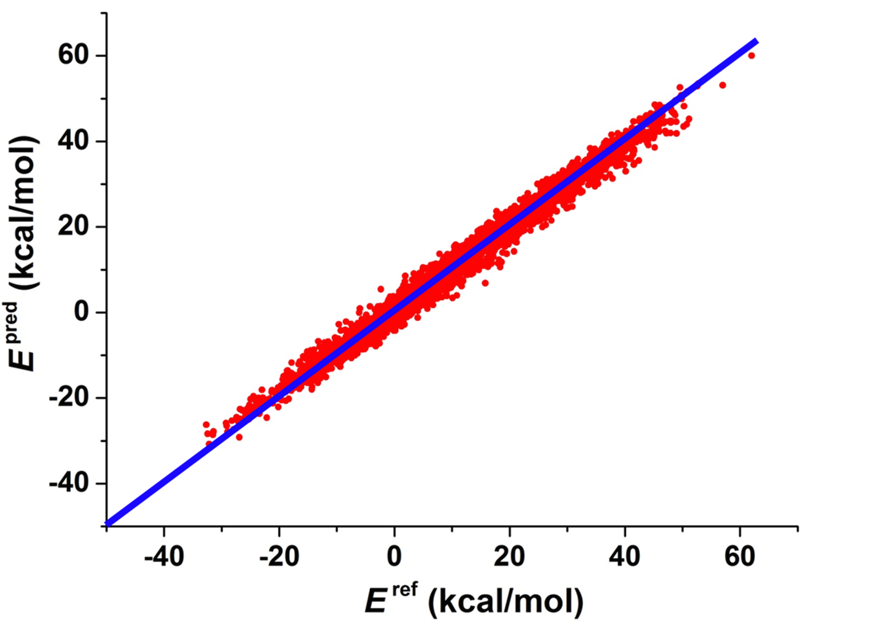
\includegraphics[height=1.5in]{figures_ml/weitao_claisen_scatter.png}  \\
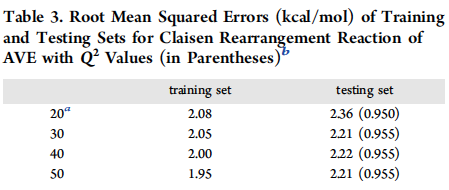
\includegraphics[height=0.9in]{figures_ml/weitao_claisen_rms.png}
\end{center} 
\end{column}
\begin{column}{0.5\textwidth}
\begin{center}
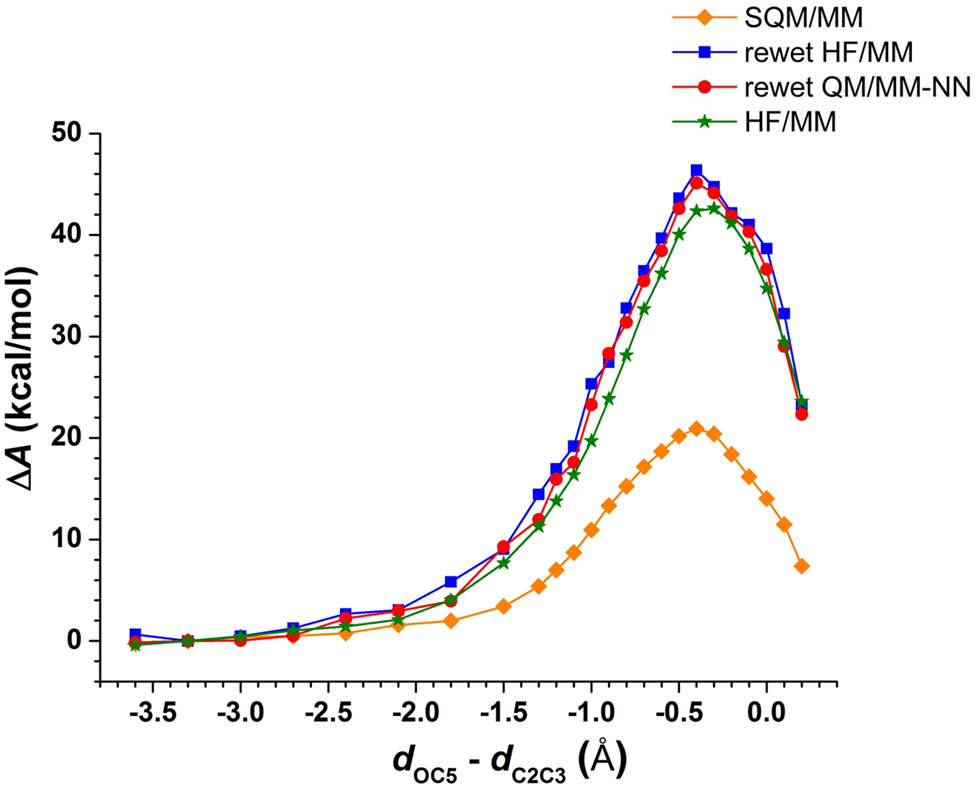
\includegraphics[height=1.8in]{figures_ml/weitao_claisen_profile.png} 
\begin{itemize}
\item \scriptsize{1ns of SQM/MM simulation per window}
\item 2000 frames are collected per window
\item QM/MM-NN 66 times faster than ``rewet HF/MM"
\end{itemize}
\end{center}
\end{column}
\end{columns}
\vspace{10mm}
\begin{center}
\footnotesize{Shen, Wu, Yang, JCTC, 12, 4934 (2016).}
\end{center} 
\end{frame}

\begin{frame}
\begin{itemize}
\item \scriptsize{Step 1: Perform 1ns SCC-DFTB/MM simulation for each US window.   Collect 200 frames. }
\item Step 2: Compute the HF/MM force for 200 frames
\item Step 3: use ML to ``learn" corrections to \textcolor{red}{the force along the reaction coordinate}
\item Step 4: Rerun the simulation with corrected SCC-DFTB/MM force.   
\item Step 5. Use WHAM to get the free energy profile.  
\end{itemize}
\begin{center}
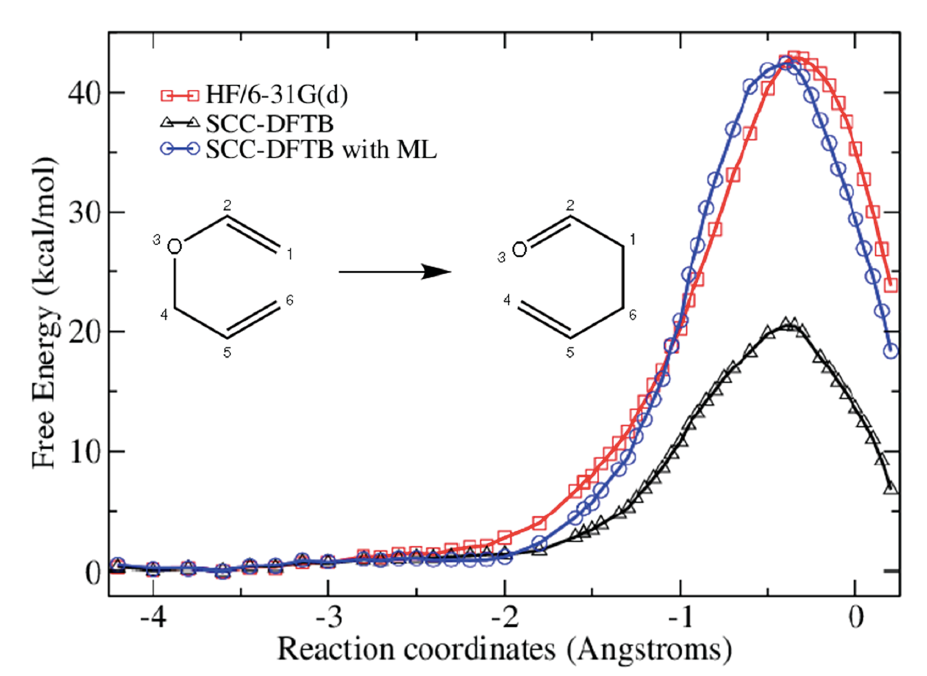
\includegraphics[height=2.2in]{figures_ml/weitao_claisen_profile2.png}
\end{center}
\vspace{1mm}
\begin{center}
\footnotesize{Wu, Shen, Yang, JCP, 147, 161732 (2017).}
\end{center} 
\end{frame}

\subsection{E(CCSD(T)) - E (MP2), Shaw (2017).}

\begin{frame}
\begin{itemize}
\item \scriptsize{3149 different chemical systems; 3---2486 configurations per system}
\item Target data: CCSD(T)/CBS-quality interaction energies using composite calculations
\item Input data: \textcolor{red}{energies, density matrix overlap} 
\end{itemize}
\begin{center}
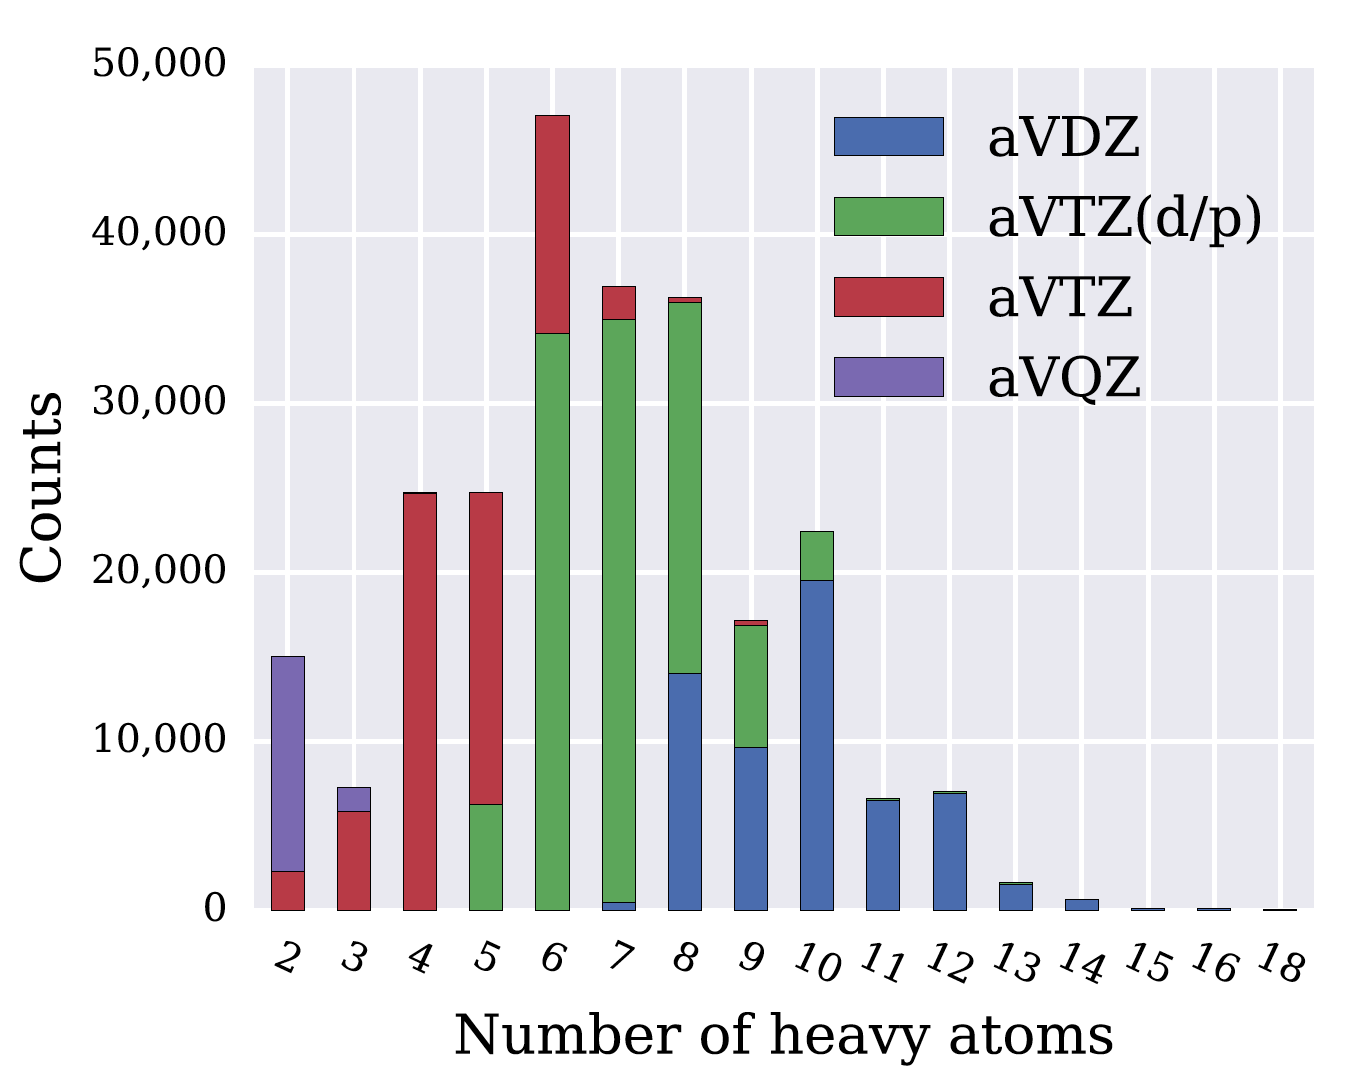
\includegraphics[height=2.2in]{figures_ml/Shaw_training.png}
\end{center}
\vspace{1mm}
\begin{center}
\footnotesize{McGibbon, $\cdots$, Klepeis, and Shaw, JCP, 147, 161725 (2017).}
\end{center} 
\end{frame}

\begin{frame}
\begin{itemize}
\item Results for S66x8 (left) and T80 (right) 
\end{itemize}

\begin{center}
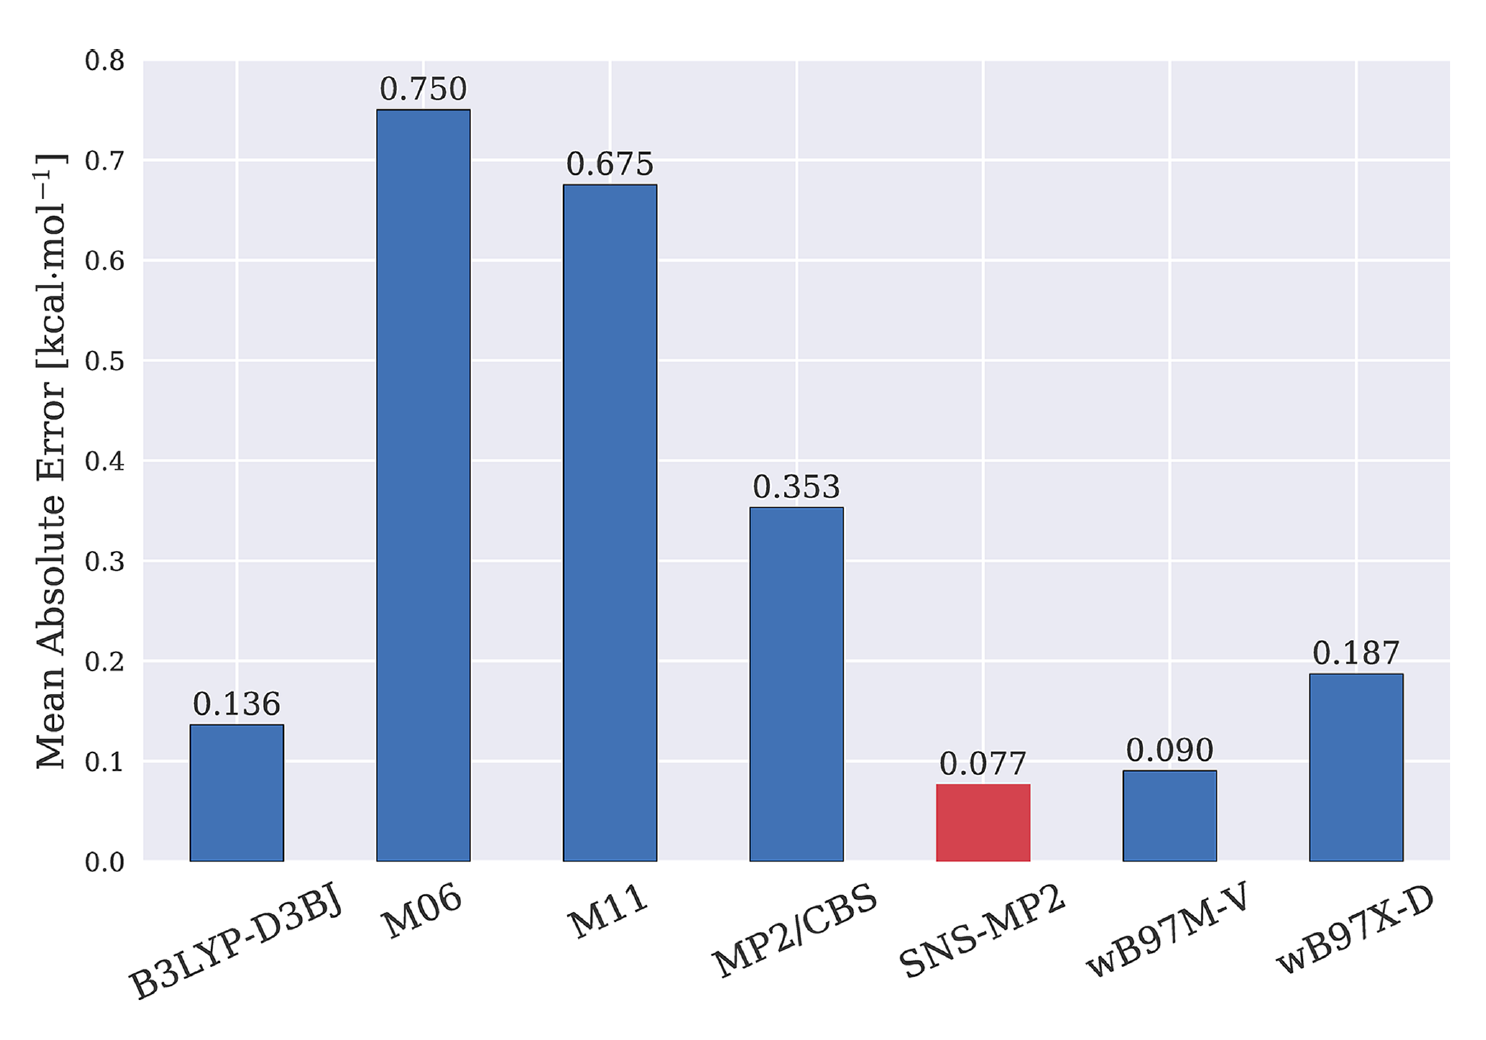
\includegraphics[height=1.6in]{figures_ml/Shaw_S66.png}
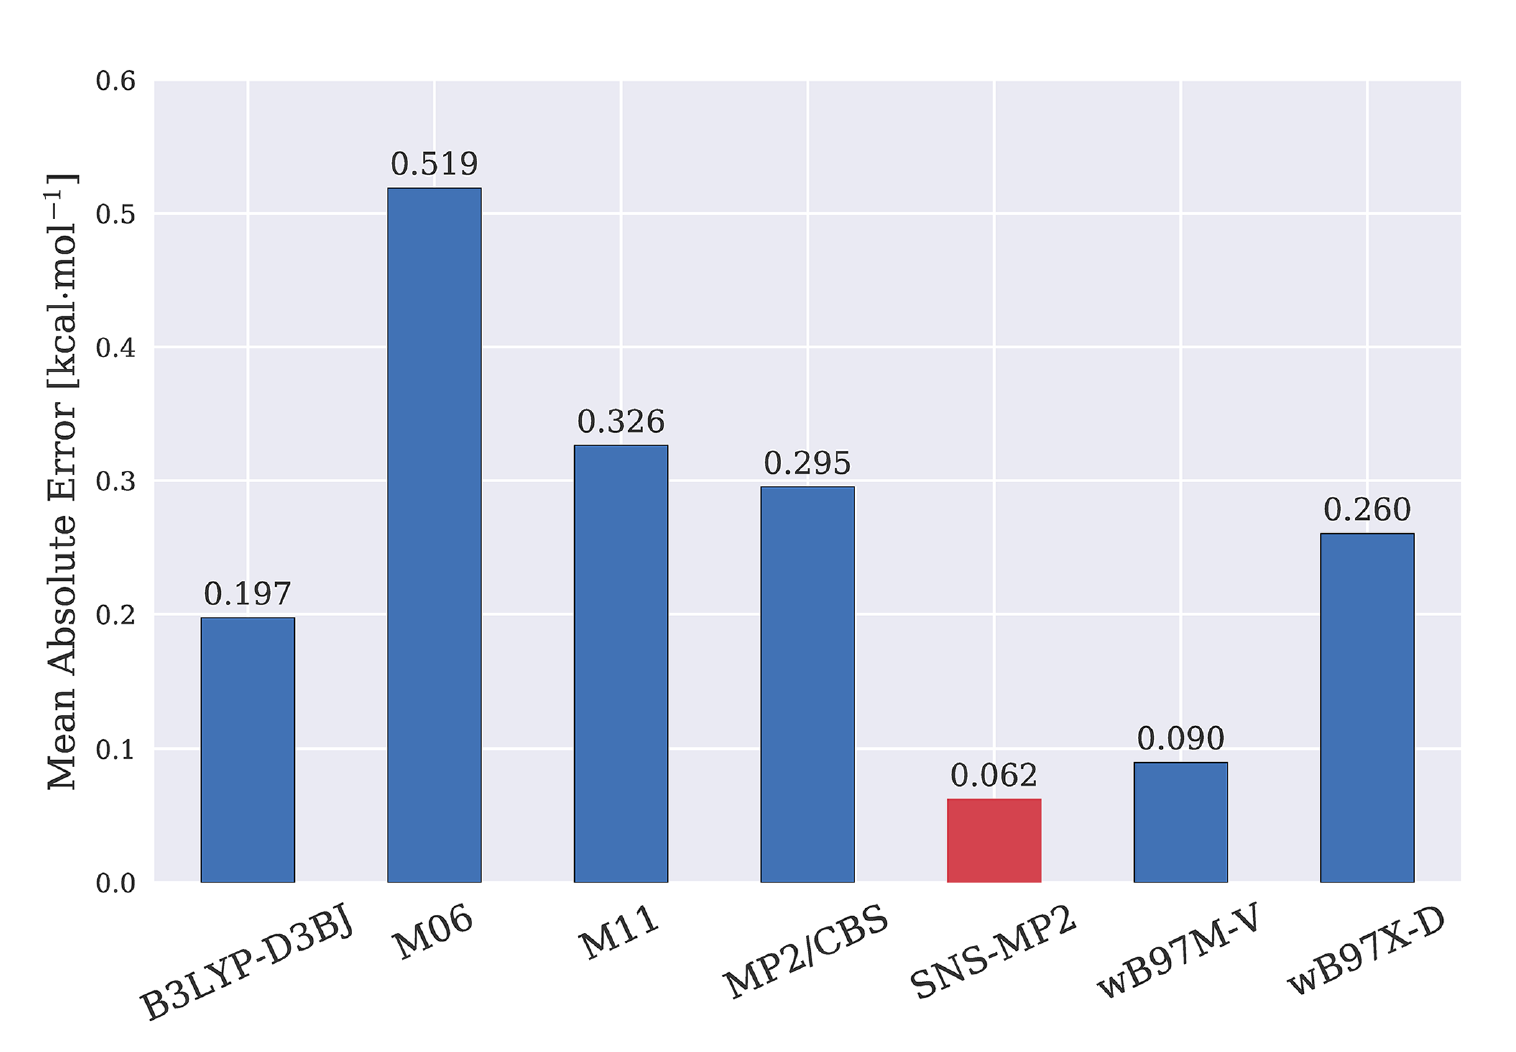
\includegraphics[height=1.6in]{figures_ml/Shaw_T80.png}
\end{center}
\vspace{10mm}
\begin{center}
\footnotesize{McGibbon, $\cdots$, Klepeis, and Shaw, JCP, 147, 161725 (2017).}
\end{center} 
\end{frame}

\subsection{$\Delta$E(CC2) - $\Delta$E (TDDFT), von Lilenfeld (2015)}

\begin{frame}

\begin{itemize}
\item \scriptsize{The prediction is} 
$\Delta E^{CC2}_i (\mathbf{d}_q) \sim \Delta E^{TDDFT}_i (\mathbf{d}_q)  + \sum_{i}^{N_{\mathrm{training}}} C_{it} e^{- \left| \mathbf{d}_q - \mathbf{d}_t \right| / \sigma} $. 
\item 20,000 organic molecules
\item Input data: coulomb matrix (with extra zero elements for small molecules); bag-of-bonds  
\end{itemize}
\begin{center}
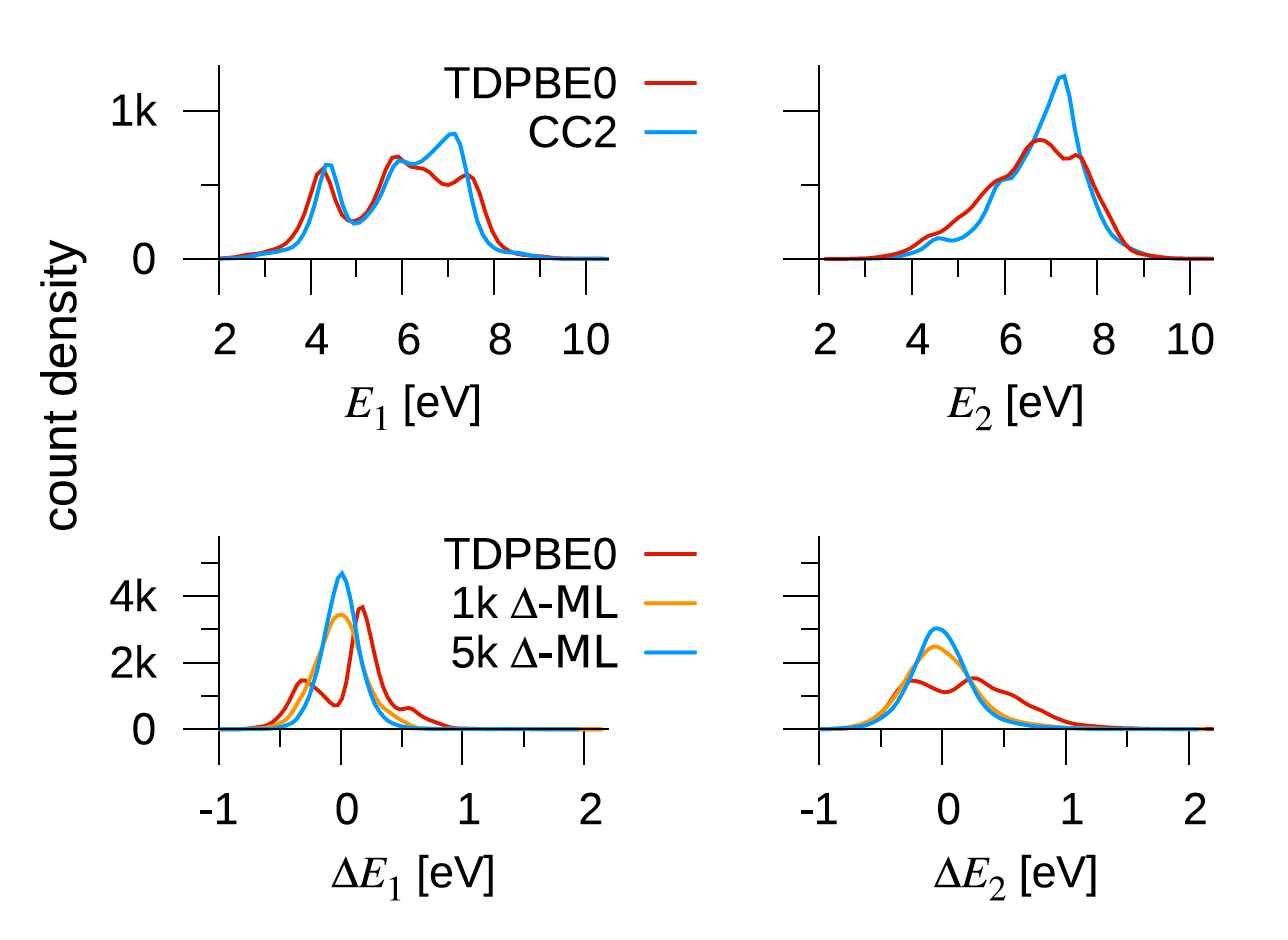
\includegraphics[height=2.2in]{figures_ml/Lilenfeld_TDDFT_dist.png}
\end{center}
\vspace{-3mm}
\begin{center}
\footnotesize{Ramakrishnan, Hartmann, Tapavicza and von Lilenfeld, JCP, 143, 084111 (2017).}
\footnotesize{See also Aspuru-Guzik et al, Chem. Sci. 7, 5139 (2016).  Error $<$ 0.01eV.} 
\end{center} 
\end{frame}

\subsection{Deformation Energy and Vibrational Analysis, Thiel (2017)}

\begin{frame}
\begin{itemize}
\item \scriptsize{CH$_3$Cl molecule, 44819 geometries}
\item descriptor: 10 atom-atom distances
\item Errors in 166 vibrational energy levels up to 5000 cm$^{-1}$ and 3606 vibrational energy levels up to 10000 cm$^{-1}$

\end{itemize}
\begin{center}
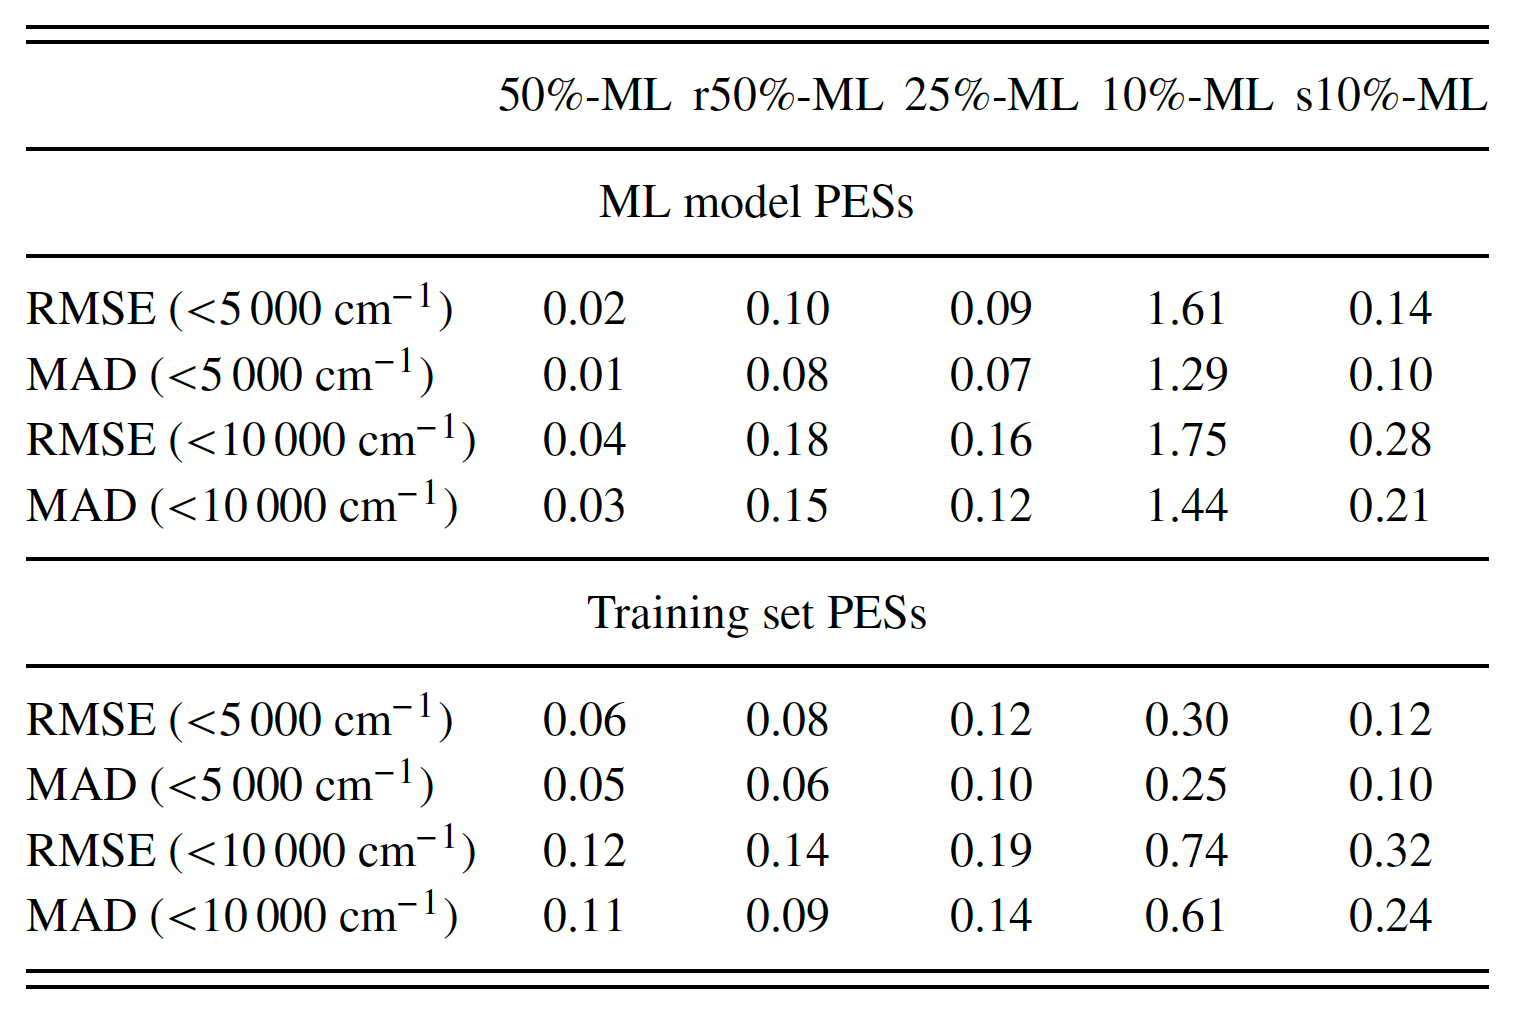
\includegraphics[height=2.2in]{figures_ml/Thiel_frequency.png}
\end{center}
\vspace{5mm}
\begin{center}
\footnotesize{Dral, Yurchenko and Thiel, 146, 244108 (2017).}
\end{center} 
\end{frame}


\section{ML Optimization of Energy Functions} 

\subsection{AMOEBA Model, Roux (2017)}

\begin{frame}
\vspace{-8mm} 
\begin{columns}
\begin{column}{0.3\textwidth}
\begin{center}
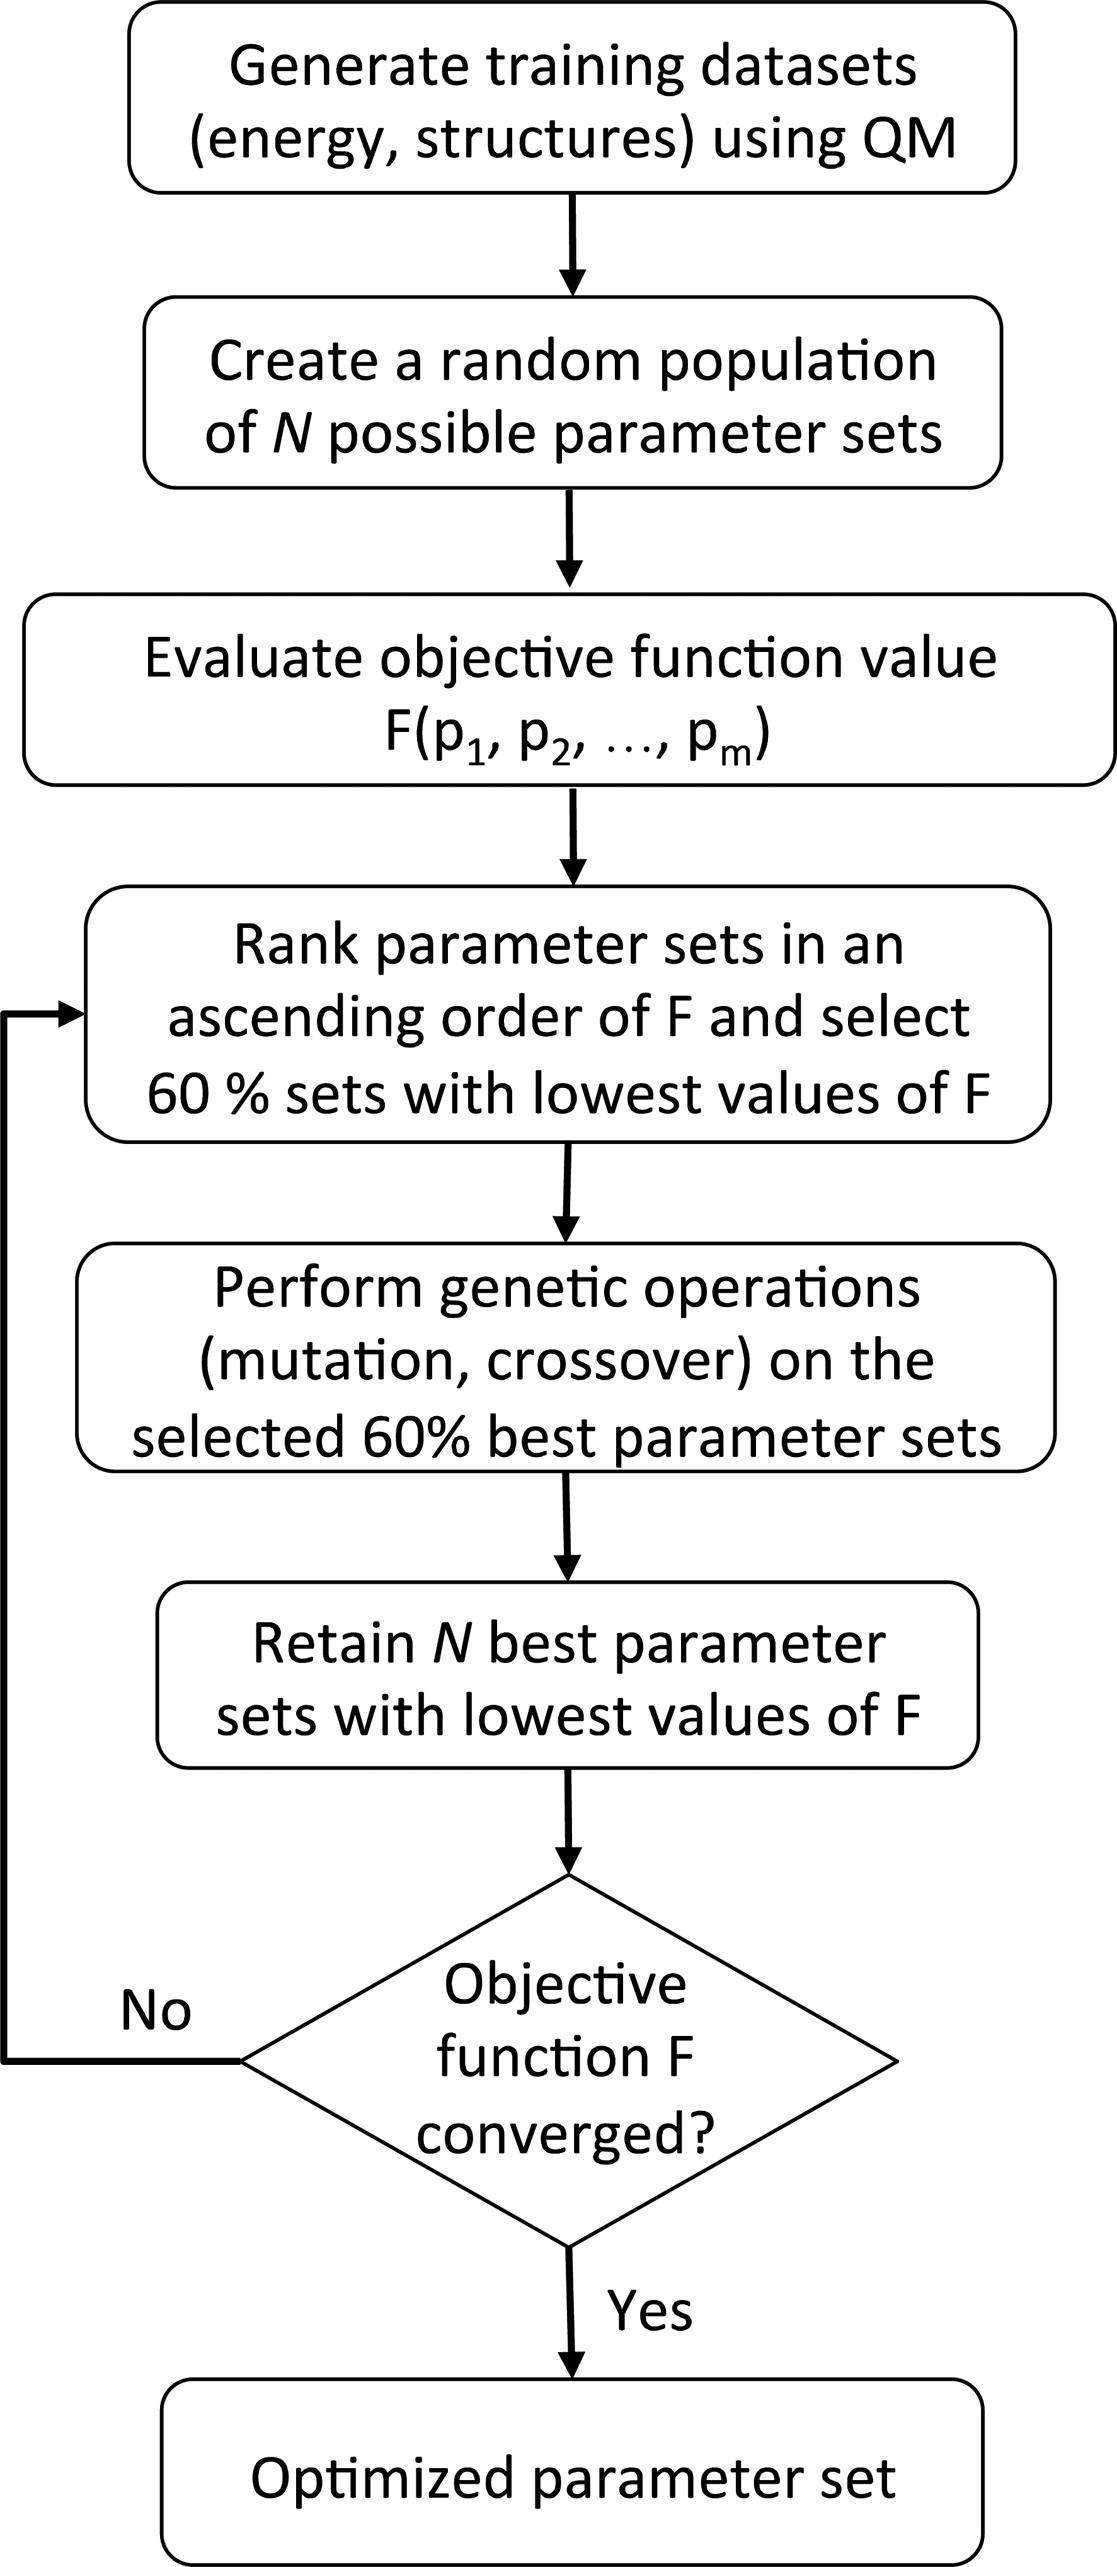
\includegraphics[height=2.4in]{figures_ml/Roux_flow.png}
\end{center}
%\vspace{5mm}
\end{column}
\begin{column}{0.7\textwidth}
\begin{center}
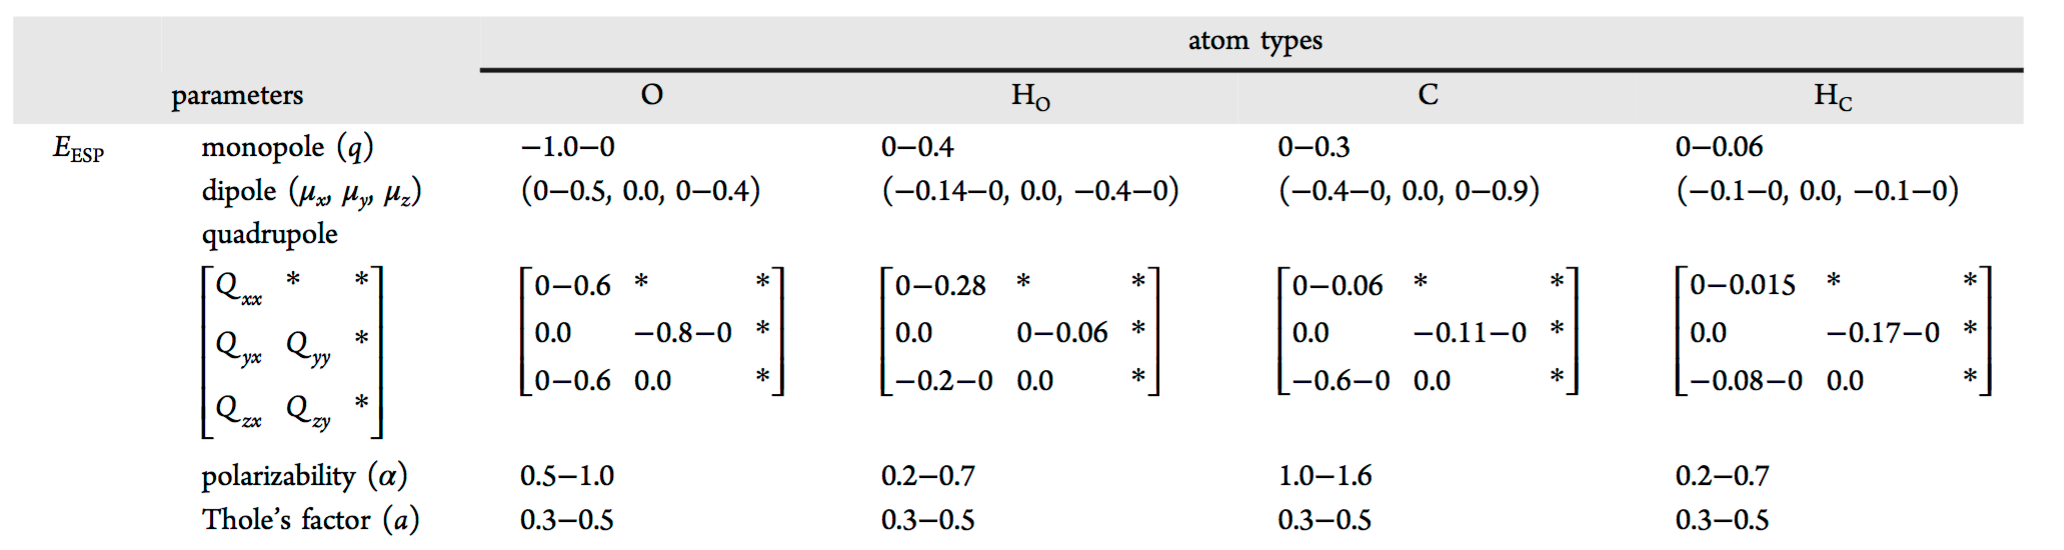
\includegraphics[height=1.2in]{figures_ml/Roux_parameters1.png} \\
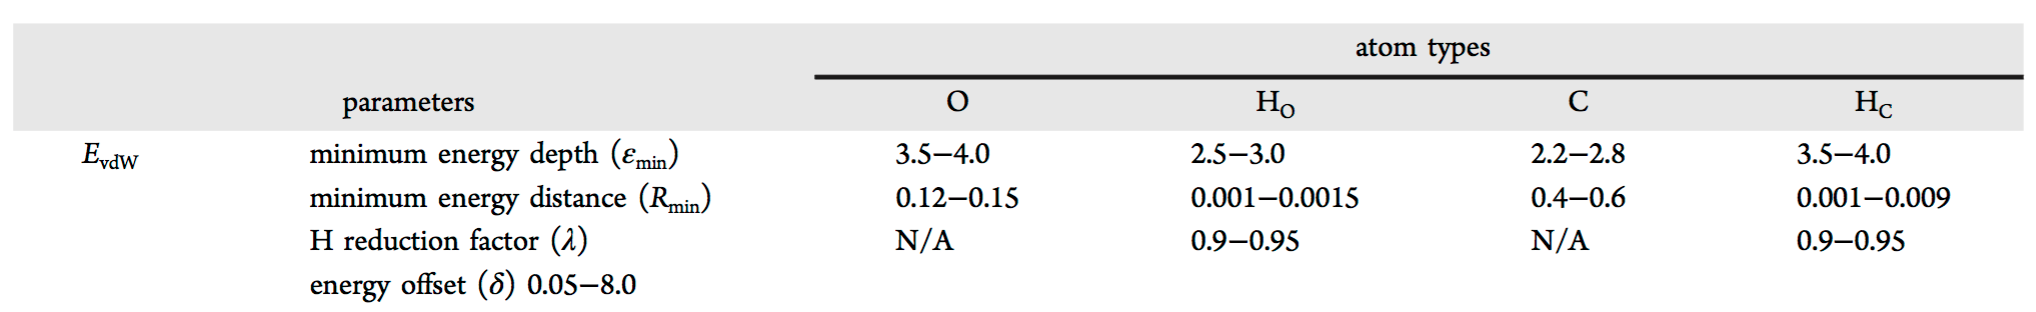
\includegraphics[height=0.7in]{figures_ml/Roux_parameters2.png} \\
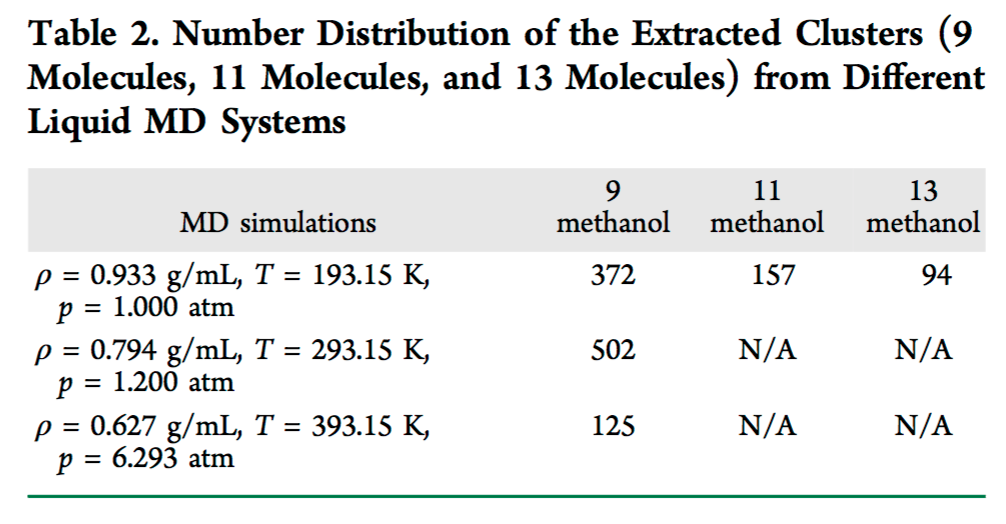
\includegraphics[height=1.2in]{figures_ml/Roux_training_set.png}
\end{center}
\end{column}
\end{columns}
\begin{center}
\scriptsize{Li, Li, Pickard, $\cdots$, Roux, Brooks, Roux, JCTC, 13, 4492 (2017).}
\end{center} 
\end{frame}


\begin{frame}
\begin{itemize}
\item \scriptsize{Interaction energy of 1250 methanol clusters} 
\end{itemize}
\begin{center}
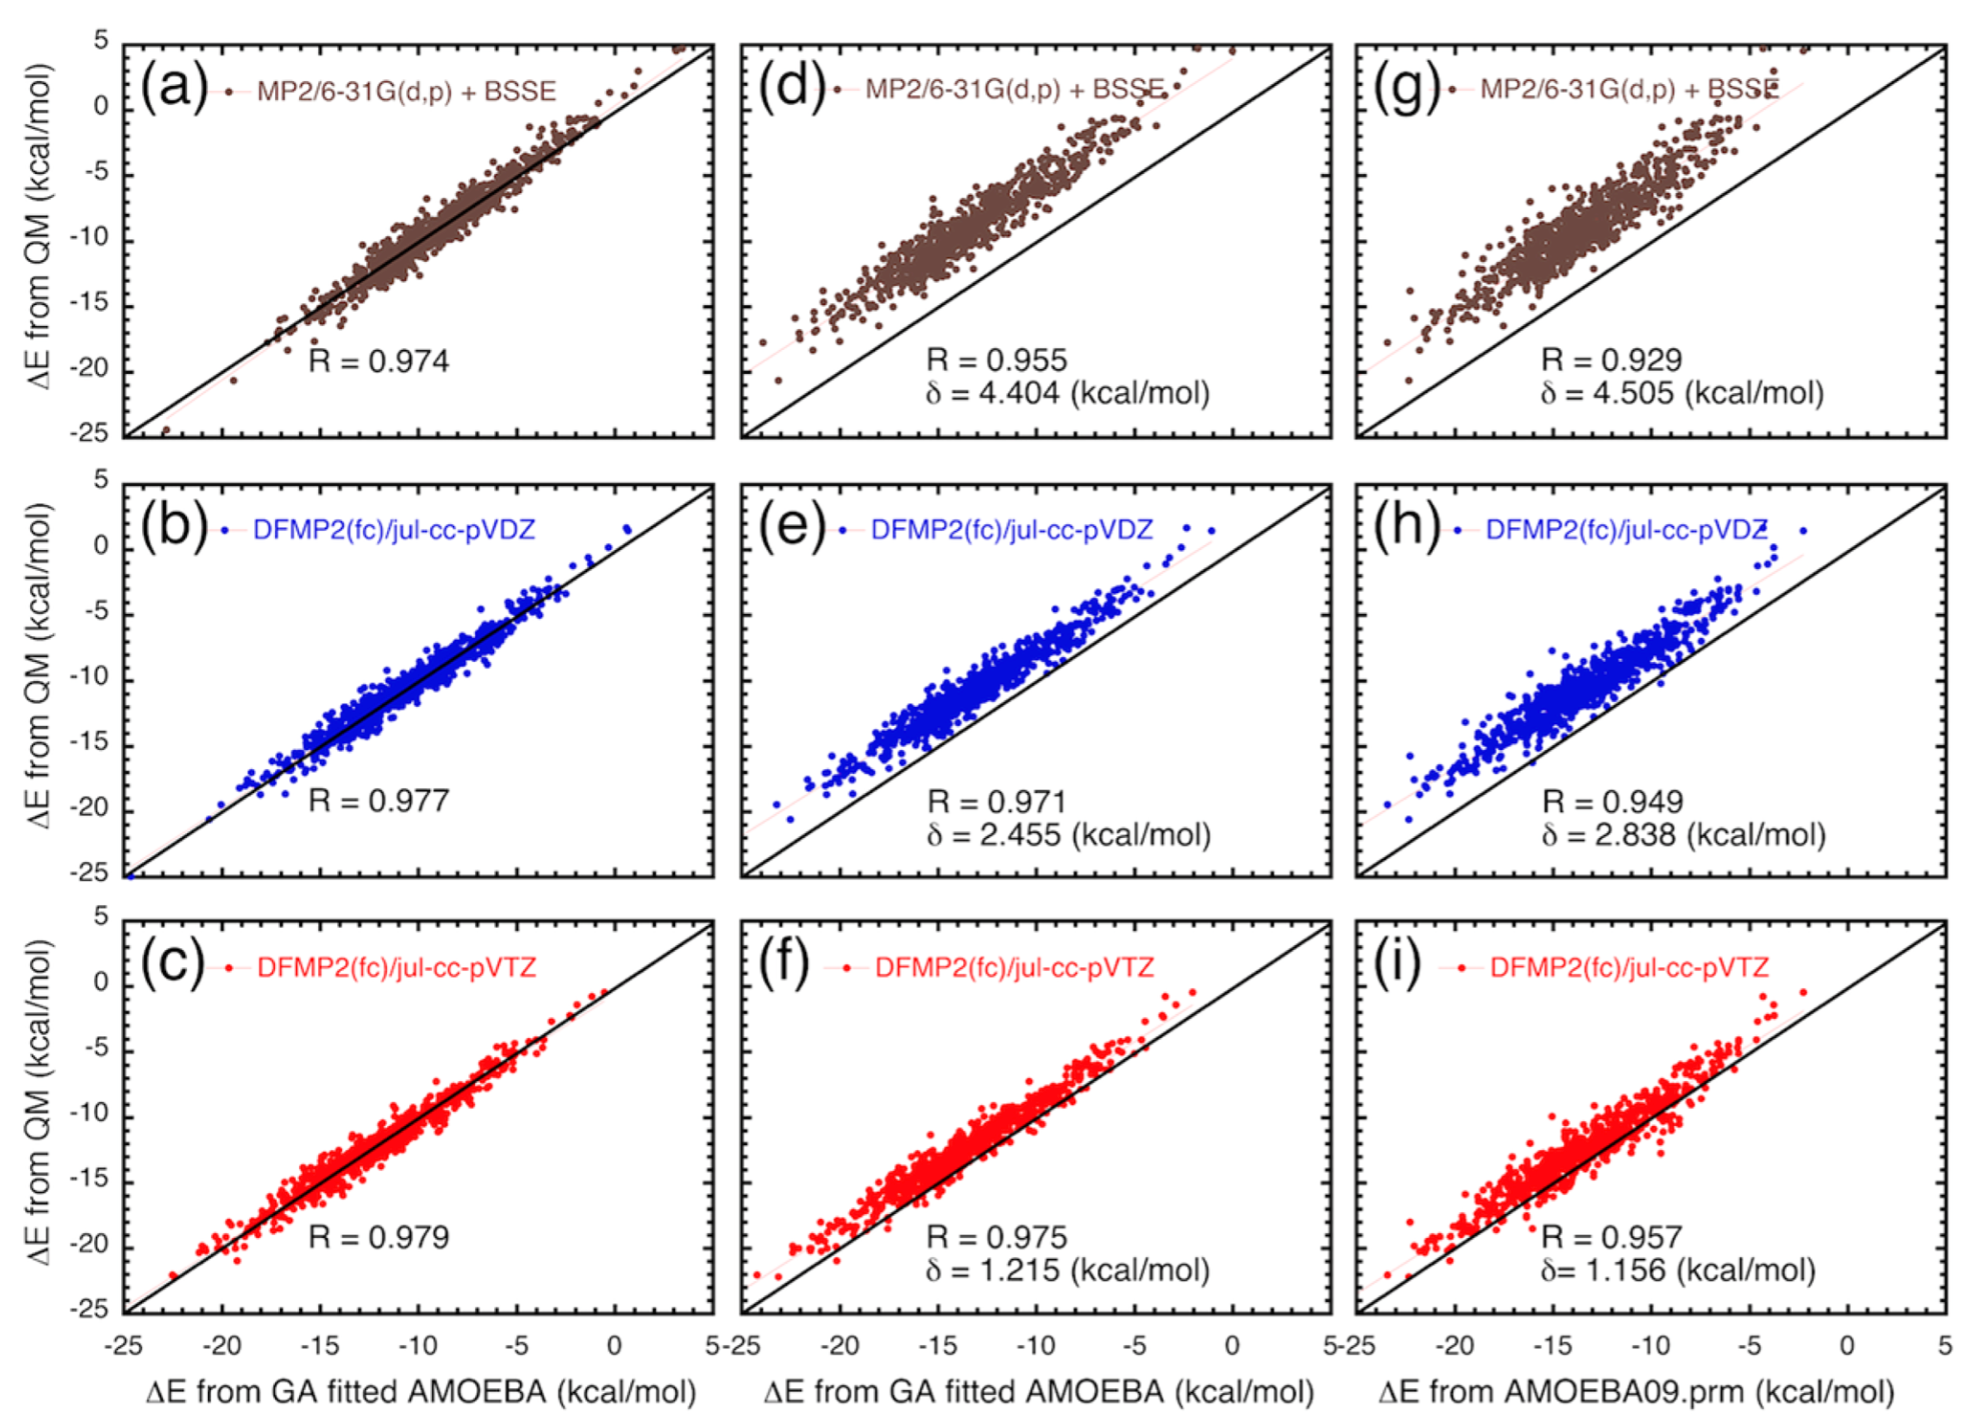
\includegraphics[height=2.4in]{figures_ml/Roux_scatter.png}
\end{center}
%\vspace{5mm}
\begin{center}
\scriptsize{Li, Li, Pickard, $\cdots$, Roux, Brooks, Roux, JCTC, 13, 4492 (2017).}
\end{center} 
\end{frame}


\begin{frame}
\begin{center}
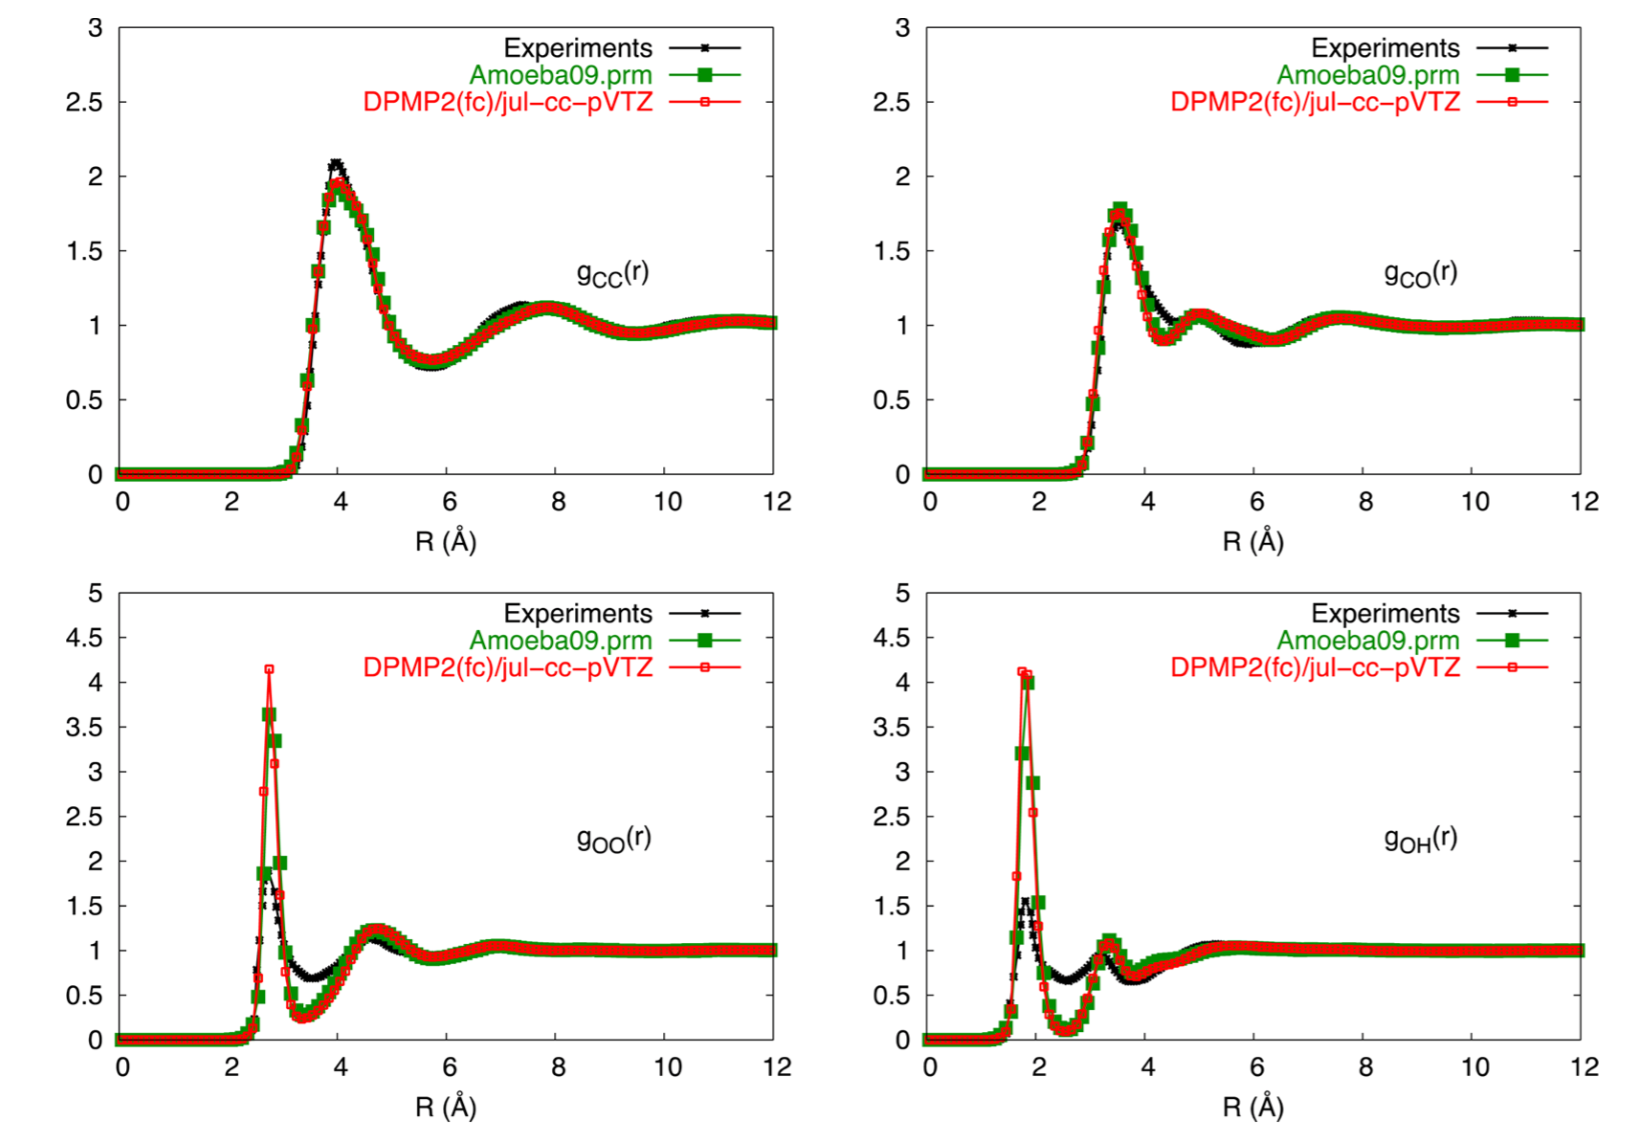
\includegraphics[height=2.4in]{figures_ml/Roux_radial.png} \\
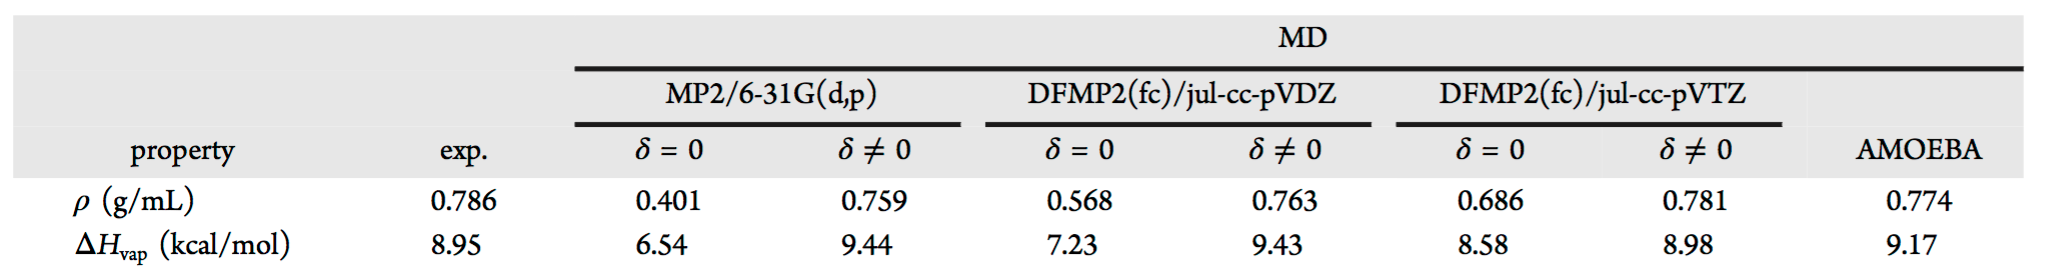
\includegraphics[height=0.6in]{figures_ml/Roux_density.png} 
\end{center}
%\vspace{5mm}
\begin{center}
\scriptsize{Li, Li, Pickard, $\cdots$, Roux, Brooks, Roux, JCTC, 13, 4492 (2017).}
\end{center} 
\end{frame}





\end{document}